\documentclass[letterpaper,12pt,fleqn]{article}
\usepackage{matharticle}
\usepackage{graphicx}
\pagestyle{empty}
\newcommand{\iid}{\overset{\text{iid}}{\sim}}
\renewcommand{\a}{\alpha}
\newcommand{\m}{\mu}
\renewcommand{\o}{\sigma}
\renewcommand{\v}{\nu}
\newcommand{\td}[2]{t_{{#1},{#2}}}
\DeclareMathOperator{\nd}{N}
\begin{document}
\section*{t Distributions}

Previously for random variables with normal distributions, \(1-\a\) confidence intervals for \(\m\) were determined when \(\m\)
is unknown but \(\o\) is known.  It is now assumed that neither \(\m\) nor \(\o\) are known.

\begin{definition}[t Distribution]
  The \emph{t distribution} with \(\v\) degrees of freedom is a continuous distribution whose pdf has the form:
  \[f(x)=C\left(1+\frac{x^2}{\v}\right)^{-\frac{v+1}{2}}\]
  for all \(x\in\R\).
\end{definition}

\begin{properties}[t Distributions]
  \begin{minipage}[t]{3in}
    \vspace{0pt}
    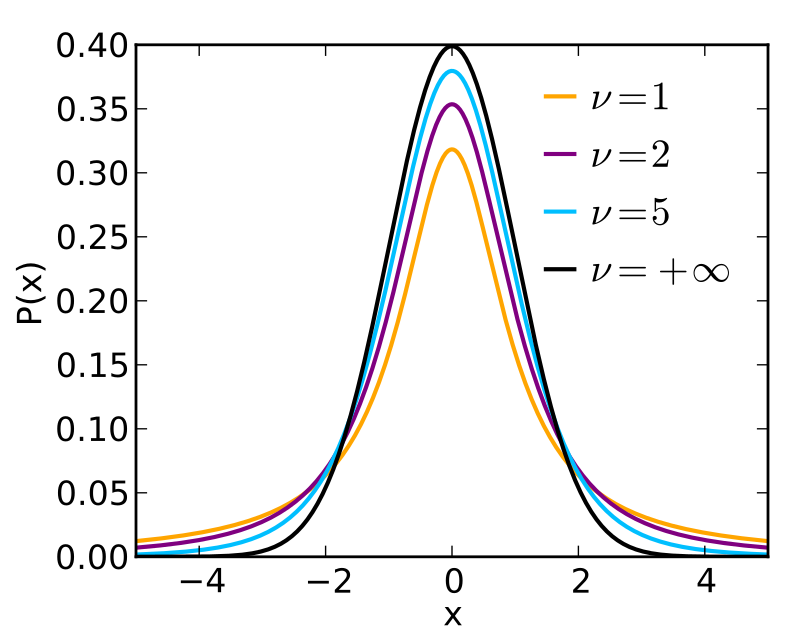
\includegraphics[scale=0.25]{tdist.png}
  \end{minipage}
  \begin{minipage}[t]{3.5in}
    \begin{enumerate}
    \setlength{\itemsep}{5pt}
    \item[]
    \item Symmetric, unimodal, and bell-shaped
    \item \(E(X)=0\)
    \item \(V(X)=\frac{v}{v-2}\quad v>2\)
    \item \(t(v)\to\nd(0,1)\) as \(v\to\infty\)
    \item Thicker tails than \(\nd(0,1)\)
    \end{enumerate}
  \end{minipage}
\end{properties}

Since \(\o\) is unknown, \(S\) will be used as a point estimate.

\begin{theorem}
  Let \(X_i\iid\nd(\m,\o^2)\) such that \(\m\) and \(\o\) are unknown:
  \[\frac{\bar{X}-\m}{\frac{S}{\sqrt{n}}}\sim T\]
  Furthermore, the \(1-\a\) confidence interval for \(\bar{X}\) is given by:
  \[\bar{x}\pm\td{\frac{\a}{2}}{n-1}\frac{s}{\sqrt{n}}\]
  where \(\td{\frac{\a}{2}}{n-1}\) is the \(\frac{\a}{2}\) critical point for the \(t\) distribution with \(n-1\) degrees
  of freedom (i.e., \(\v=n-1\)).
\end{theorem}

\begin{example}
  A sample carton of brown eggs from a farm has \(\bar{x}=65.5\) and \(s^2=4.69\).  Assuming a normal population with
  unknown variance, obtain the 95\% confidence interval.
  \begin{gather*}
    1-\a=0.95 \\
    \a=1-0.95=0.05 \\
    \frac{\a}{2}=\frac{0.05}{2}=0.025
    \td{0.025}{11}=2.201
    \\
    \bar{x}\pm\td{0.025}{11}\frac{s}{\sqrt{n}}=65.5\pm2.201\sqrt{\frac{4.69}{12}}=65.5\pm1.4=(64.1,66.9)
  \end{gather*}
\end{example}

\end{document}
